\section{Chapter Prerequisites --- Conic Sections}
\label{sec:conic_sections}

\prereqIntro

The ancient Greeks recognized that interesting shapes can be formed by intersecting a plane with a 
\textit{double napped} cone (i.e., two identical cones placed tip--to--tip as shown in the following figures). As these shapes are formed as sections of conics, they have earned the official name ``conic sections.''

The three ``most interesting'' conic sections are given in the top row of \autoref{fig:nondeg_conic}. They are the parabola, the ellipse (which includes circles) and the hyperbola. In each of these cases, the plane does not intersect the tips of the cones (usually taken to be the origin).

\begin{lxfigure}
\flushinner{%
\small
\begin{tabular}{cccc}
\myincludegraphics[scale=.25]{figures/conic_parabola}&
\myincludegraphics[scale=.25]{figures/conic_ellipse}&
\myincludegraphics[scale=.25]{figures/conic_circle}&
\myincludegraphics[scale=.25]{figures/conic_hyperbola} \\
Parabola & Ellipse & Circle &  Hyperbola \\
\myincludegraphics[scale=.25]{figures/conic_singlept}&
\myincludegraphics[scale=.25]{figures/conic_oneline}&
\myincludegraphics[scale=.25]{figures/conic_crossedlines} \\
Point & Line & Crossed Lines 
\end{tabular}}
\caption{Conic Sections}\label{fig:nondeg_conic}
\end{lxfigure}
% todo convert conic figures to asymptote (or at least tikz)

When the plane does contain the origin, three \textbf{degenerate} cones can be formed as shown the bottom row of \autoref{fig:nondeg_conic}: a point, a line, and crossed lines. We focus here on the nondegenerate cases.\index{conic sections}\index{conic sections!degenerate}

While the above geometric constructs define the conics in an intuitive, visual way, these constructs are not very helpful when trying to analyze the shapes algebraically or consider them as the graph of a function. It can be shown that all conics can be defined by the general second--degree equation
\[Ax^2+Bxy+Cy^2+Dx+Ey+F=0.\]
While this algebraic definition has its uses, most find another geometric perspective of the conics more beneficial.

Each nondegenerate conic can be defined as the \textbf{locus}, or set, of points that satisfy a certain distance property. These distance properties can be used to generate an algebraic formula, allowing us to study each conic as the graph of a function.

\subsection{Parabolas}

\definition{def:parabola}{Parabola}
{A \textbf{parabola} is the locus of all points equidistant from a point (called a \textbf{focus}) and a line (called the \textbf{directrix}) that does not contain the focus.
\index{conic sections!parabola}\index{parabola!definition}\index{directrix}\index{focus}
}

\mtable{Illustrating the definition of the parabola and establishing an algebraic formula.}{fig:parabola_def}{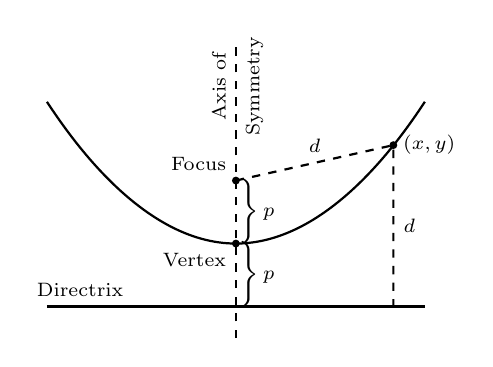
\begin{tikzpicture}[scale=.8]
	\draw [thick,draw={\colorone}] (-3,-1)
	 node [above,black,shift={(12pt,0pt)}] {\scriptsize Directrix}
	 -- (3,-1);
	\filldraw [black] (0,1) circle (1.5pt) node [above left] {\scriptsize Focus};
	\draw [thick,draw={\colortwo}](-3,2.25) parabola bend (0,0) (3,2.25);
	\filldraw (0,0) circle (1.5pt) node [below left] {\scriptsize Vertex};
	\draw (.3,.5) node[] {\scriptsize $\left.\rule{0pt}{12pt}\right\}p$};
	\draw (.3,-.5) node[] {\scriptsize $\left.\rule{0pt}{12pt}\right\}p$};
	\coordinate (A) at (2.5,1.5625);
	\filldraw [black] (A) circle (1.5pt) node [right] {\scriptsize $(x,y)$};
	\draw [thick,dashed](0,1) -- (A) node [pos=.5,above] {\scriptsize $d$}
	 -- (2.5,-1) node [pos=.5,right] {\scriptsize $d$};
	\draw [thick,dashed] (0,-1.5) -- node [pos=.85,above,rotate=90]
	 {\scriptsize Axis of}
	 node [pos=.85,below,rotate=90] {\scriptsize Symmetry} (0,3.2);
\end{tikzpicture}}

\autoref{fig:parabola_def} illustrates this definition. The point halfway between the focus and the directrix is the \textbf{vertex}. The line through the focus, perpendicular to the directrix, is the \textbf{axis of symmetry}, as the portion of the parabola on one side of this line is the mirror--image of the portion on the opposite side.

\ifthenelse{\boolean{abridgeConics}}{}{%
The definition leads us to an algebraic formula for the parabola. Let $P=(x,y)$ be a point on a parabola whose focus is at $F=(0,p)$ and whose directrix is at $y=-p$. (We'll assume for now that the focus lies on the $y$-axis; by placing the focus $p$ units above the $x$-axis and the directrix $p$ units below this axis, the vertex will be at $(0,0)$.)

We use the Distance Formula to find the distance $d_1$ between $F$ and $P$:
\[d_1=\sqrt{(x-0)^2+(y-p)^2}.\]
The distance $d_2$ from $P$ to the directrix is more straightforward:
\[d_2=y-(-p) = y+p.\]
These two distances are equal. Setting $d_1=d_2$, we can solve for $y$ in terms of $x$:
\begin{align*}
	d_1&= d_2 \\
	\sqrt{x^2+(y-p)^2} &= y+p 
	\intertext{Now square both sides.}
	x^2+(y-p)^2 &= (y+p)^2 \\
	x^2+y^2-2yp+p^2 &= y^2+2yp+p^2\\
	x^2 &=4yp\\
	y&= \frac{1}{4p}x^2.
\end{align*}%
}
The geometric definition of the parabola and distance formula can be used to derive the quadratic function whose graph is a parabola with vertex at the origin.
\[y=\frac{1}{4p}x^2.\]
Applying transformations of functions we get the following standard form of the parabola.

\keyidea{idea:parabola}{General Equation of a Parabola}
{\begin{enumerate}
	\item	\textbf{Vertical Axis of Symmetry:} The equation of the parabola with vertex at $(h,k)$, directrix $y=k-p$, and focus at $(h,k+p)$ in standard form is \[y=\frac{1}{4p}(x-h)^2+k.\]
	\item	\textbf{Horizontal Axis of Symmetry:} The  equation of the parabola with vertex at $(h,k)$, directrix $x=h-p$, and focus at $(h+p,k)$ in standard form is \[x=\frac{1}{4p}(y-k)^2+h.\]
\end{enumerate}
Note: $p$ is not necessarily a positive number.\index{parabola!general equation}}

\example{ex_conic1}{Finding the equation of a parabola}{Give the equation of the parabola with focus at $(1,2)$ and directrix at $y=3$.}
{The vertex is located halfway between the focus and directrix, so $(h,k) = (1,2.5)$. This gives $p=-0.5$. Using \autoref{idea:parabola} we have the equation of the parabola as
%
\mtable{The parabola described in \autoref{ex_conic1}.}{fig:conic1}{\begin{tikzpicture}
\begin{axis}[width=1.16\marginparwidth,tick label style={font=\scriptsize},
axis y line=middle,axis x line=middle,name=myplot,axis equal,
ymin=-6.5,ymax=2.9,xmin=-3.5,xmax=5.5]
\addplot [thick, draw={\colorone},smooth,domain=-3:5] {-.5*(x-1)^2+2.5};
\end{axis}
\node [right] at (myplot.right of origin) {\scriptsize $x$};
\node [above] at (myplot.above origin) {\scriptsize $y$};
\end{tikzpicture}}
%
\[y=\frac{1}{4(-0.5)}(x-1)^2+2.5 = -\frac12(x-1)^2+2.5.\]
The parabola is sketched in \autoref{fig:conic1}.}

\ifthenelse{\boolean{abridgeConics}}{}{%
\example{ex_conic2}{Finding the focus and directrix of a parabola}{Find the focus and directrix of the parabola $x=\frac18y^2-y+1$. The point $(7,12)$ lies on the graph of this parabola; verify that it is equidistant from the focus and directrix.}
{We need to put the equation of the parabola in its general form. This requires us to complete the square:
\begin{align*}
	x &= \frac18y^2-y+1 \\
	&= \frac18\big(y^2-8y+8\big)\\
	&=	\frac18\big(y^2-8y+16 -16+8\big)\\
	&=	\frac18\big((y-4)^2 - 8\big)\\
	&=	\frac18(y-4)^2 -1.
\end{align*}
Hence the vertex is located at $(-1,4)$.  We have $\frac18=\frac1{4p}$, so $p=2$. We conclude that the focus is located at $(1,4)$ and the directrix is  $x=-3$. The parabola is graphed in \autoref{fig:conic2}, along with its focus and directrix.\bigskip

\mtable{The parabola described in \autoref{ex_conic2}. The distances from a point on the parabola to the focus and directrix is given.}{fig:conic2}{\begin{tikzpicture}
\begin{axis}[width=1.16\marginparwidth,tick label style={font=\scriptsize},
axis y line=middle,axis x line=middle,name=myplot,xtick={-10,-5,5,10},
ymin=-5.5,ymax=14.5,xmin=-11,xmax=14,axis equal]
\addplot [thick, draw={\colorone},smooth,domain=-5:14] ({x^2/8-x+1},x);
\addplot [thick, draw={\colortwo},smooth,domain=-5:14] (-3,x);
\draw [dashed,draw={\colorone!70},thick] (axis cs:-3,12)
 -- node [above,pos=.5,black] {\scriptsize 10} (axis cs:7,12)
 -- node [pos=.6,right,black] {\scriptsize 10} (axis cs: 1,4);
\filldraw [draw={\colortwo}] (axis cs: 1,4) circle (1.5pt)
 (axis cs: 7,12) circle (1.5pt);
\end{axis}
\node [right] at (myplot.right of origin) {\scriptsize $x$};
\node [above] at (myplot.above origin) {\scriptsize $y$};
\end{tikzpicture}}

The point $(7,12)$ lies on the graph and is $7-(-3)=10$ units from the directrix. The distance from $(7,12)$ to the focus is:
\[\sqrt{(7-1)^2 + (12-4)^2} = \sqrt{100}=10.\]
Indeed, the point on the parabola is equidistant from the focus and directrix.}
	
\subsection{Reflective Property}

One of the fascinating things about the nondegenerate conic sections is their reflective properties. Parabolas have the following reflective property:

\begin{quote}
	Any ray emanating from the focus that intersects the parabola reflects off along a line perpendicular to the directrix.
\end{quote}

This is illustrated in \autoref{fig:conic_reflect}. The following theorem states this more rigorously.

\mtable{Illustrating the parabola's reflective property.}{fig:conic_reflect}{\begin{tikzpicture}
\begin{axis}[width=1.16\marginparwidth,tick label style={font=\scriptsize},
axis y line=none,axis x line=none,name=myplot,axis equal,
ymin=-6.5,ymax=14.5,xmin=-4,xmax=12]
\coordinate (focus) at (axis cs: 1,4);
\addplot [very thick, draw={\colorone},smooth,domain=-6:14] ({x^2/8-x+1},x);
\addplot [very thick, draw={\colortwo},smooth,domain=-6:14] (-3,x);
\draw [thick](axis cs: 12,12) -- (axis cs: 7,12) -- (focus)
			(axis cs: 12,8) -- (axis cs: 1,8) -- (focus)
			(axis cs: 12,3) -- (axis cs: -.875,3)
			(axis cs: -.875,3)-- (focus)
			(axis cs: 12,-3) -- (axis cs: 5.125,-3) -- (focus);
\filldraw [draw={\colortwo}] (focus) circle (1.5pt);
\end{axis}
\end{tikzpicture}}
	
\theorem{thm:parabola_reflect}{Reflective Property of the Parabola}
{Let $P$ be a point on a parabola. The tangent line to the parabola at $P$ makes equal angles with the following two lines:
\begin{enumerate}
	\item	The line containing $P$ and the focus $F$, and
	\item	The line perpendicular to the directrix through $P$.
	\index{parabola!reflective property}
\end{enumerate}}

% todo prove the reflective property of parabolas

Because of this reflective property, paraboloids (the 3D analogue of parabolas) make for useful flashlight reflectors as the light from the bulb, ideally located at the focus, is reflected along parallel rays. Satellite dishes also have paraboloid shapes. Signals coming from satellites effectively approach the dish along parallel rays. The dish then \textit{focuses} these rays at the focus, where the sensor is located.
}

\subsection{Ellipses}

\definition{def:ellipse}{Ellipse}
{An \textbf{ellipse} is the locus of all points whose sum of distances from two fixed points, each a \textbf{focus} of the ellipse, is constant.\index{conic sections!ellipse}\index{ellipse!definition}\index{focus}}

An easy way to visualize this construction of an ellipse is to pin both ends of a string to a board. The pins become the foci. Holding a pencil tight against the string places the pencil on the ellipse; the sum of distances from the pencil to the pins is constant: the length of the string. See \autoref{fig:ellipse_def}.

\ifthenelse{\boolean{abridgeConics}}{}{%
We can again find an algebraic equation for an ellipse using this geometric definition. Let the foci be located along the $x$-axis, $c$ units from the origin. Let these foci be labeled as $F_1 = (-c,0)$ and $F_2=(c,0)$. Let $P=(x,y)$ be a point on the ellipse. The sum of distances from $F_1$ to $P$ ($d_1$) and from $F_2$ to $P$ ($d_2$) is a constant $d$. That is, $d_1+d_2=d$. Using the Distance Formula, we have 
\[\sqrt{(x+c)^2+y^2} + \sqrt{(x-c)^2+y^2} = d.\]
Using a fair amount of algebra can produce the following equation of an ellipse (note that the equation is an implicitly defined function; it has to be, as an ellipse fails the Vertical Line Test):
\[
\frac{x^2}{\left(\frac d2\right)^2} + \frac{y^2}{\left(\frac d2\right)^2-c^2} = 1.
\]
This is not particularly illuminating, but by making the substitution $a=d/2$ and $b=\sqrt{a^2-c^2}$, we can rewrite the above equation as 
\[\frac{x^2}{a^2} + \frac{y^2}{b^2} = 1.\]
}

As shown in \autoref{fig:ellipse_label}, the values of $a$ and $b$ have
% geometric
meaning. In general, the two foci of an ellipse lie on the \textbf{major axis} of the ellipse, and the midpoint of the segment joining the two foci is the \textbf{center}. The major axis intersects the ellipse at two points, each of which is a \textbf{vertex}. The line segment through the center and perpendicular to the major axis is the \textbf{minor axis}. The ``constant sum of distances'' that defines the ellipse is the length of the major axis, i.e., $2a$.
%
% this is not the figure that was just referenced, but the figure from before the previous paragraph.  But I can't get TeX to realize what page it goes on otherwise
\mtable[-6\baselineskip]{Illustrating the construction of an ellipse with pins, pencil and string.}{fig:ellipse_def}{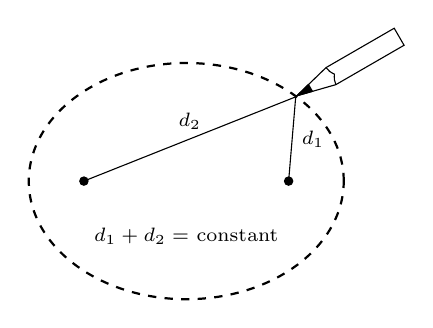
\begin{tikzpicture}
	\draw [thick,dashed] (0,0) circle [x radius=2,y radius=1.5];
	\filldraw (1.3,0)circle(1.5pt) (-1.3,0)circle(1.5pt);
	\draw  (1.3,0) -- node [right,pos=.5] {\scriptsize $d_1$}
	 (1.39,1.07) -- node [above,pos=.5] {\scriptsize $d_2$} (-1.3,0);
	\draw (0,-.7) node {\scriptsize $d_1+d_2=$ constant};
	\begin{scope}[shift={(1.9cm,1.225cm)},rotate=120,xscale=.25,yscale=.5]
		\draw (0,0) -- (0,-2) -- (1,-2)--(1,0) -- (.5,1) -- cycle;
		\draw [fill=black] (.3,.6) -- ( .5,1)--(.7,.6)--cycle;
		\draw (0,0) cos (.5,-.1) sin (1,0);
	\end{scope}
\end{tikzpicture}}

\mtable{Labeling the significant features of an ellipse.}{fig:ellipse_label}{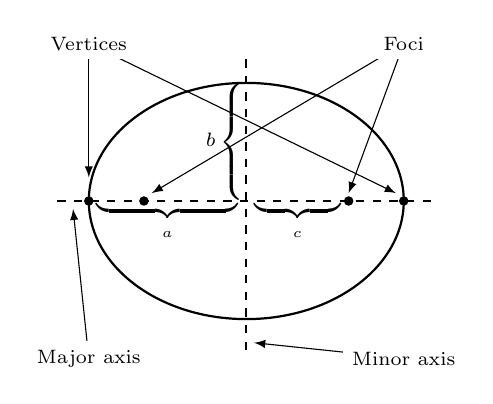
\begin{tikzpicture}
 \draw [thick,draw={\colorone}] (0,0) circle [x radius=2,y radius=1.5];
 \draw [thick,dashed] (-2.4,0) -- (2.4,0) (0,1.8) -- (0,-1.9);
 \filldraw [draw={\colortwo}] (1.3,0) circle (1.5pt) (-1.3,0) circle (1.5pt);
 \draw [->,>=latex] (-2,-2) node [fill=white] {\scriptsize Major axis}
  -- (-2.2,-.1);
 \draw [->,>=latex] (2,-2) node [fill=white] {\scriptsize Minor axis}
  -- (.1,-1.8);
 \draw [->,>=latex] (-2,2)  -- (-2,.3);
 \draw [->,>=latex] (-2,2) node [fill=white] {\scriptsize Vertices} -- (1.9,.1);
 \draw [->,>=latex] (2,2)  -- (-1.2,.1);
 \draw [->,>=latex] (2,2) node [fill=white] {\scriptsize Foci} -- (1.3,.1);
 \filldraw [draw={\colorone}] (2,0) circle (1.5pt) (-2,0) circle (1.5pt);
 \draw (-1,-.25) node {\scriptsize $\underbrace{\rule{1.8cm}{0pt}}_a$};
 \draw (.65,-.25) node {\scriptsize $\underbrace{\rule{1.1cm}{0pt}}_c$};
 \draw (-.25,.75) node [] {\scriptsize $b\left\{\rule[-.65cm]{0pt}{1.3cm}\right.$};
\end{tikzpicture}}

Allowing for the shifting of the ellipse gives the following standard equations.
	
\keyidea{idea:ellipse}{Standard Equation of the Ellipse}
{The equation of an ellipse centered at $(h,k)$ with major axis of length $2a$ and minor axis of length $2b$ in standard form is:
\begin{enumerate}
	\item	\textbf{Horizontal major axis:} $\ds \frac{(x-h)^2}{a^2}+\frac{(y-k)^2}{b^2}=1.$
	\item	\textbf{Vertical major axis:} $\ds \frac{(x-h)^2}{b^2}+\frac{(y-k)^2}{a^2}=1.$
\end{enumerate}
The foci lie along the major axis, $c$ units from the center, where $c^2=a^2-b^2$.
\index{ellipse!standard equation}}

\example{ex_conic3}{Finding the equation of an ellipse}{Find the general equation of the ellipse graphed in \autoref{fig:conic3}.
%
\mtable{The ellipse used in \autoref{ex_conic3}.}{fig:conic3}{\begin{tikzpicture}
\begin{axis}[width=1.16\marginparwidth,tick label style={font=\scriptsize},
axis y line=middle,axis x line=middle,name=myplot,xtick={-6,-4,-2,2,4,6},
ytick={-4,-2,2,4,6},ymin=-4.9,ymax=6.9,xmin=-6.9,xmax=6.9]
\addplot [thick, draw={\colorone},smooth,domain=0:360,samples=60]
 ({2*cos(x)-3},{5*sin(x)+1});
\filldraw (axis cs:-3,1)  circle (1.5pt);
\end{axis}
\node [right] at (myplot.right of origin) {\scriptsize $x$};
\node [above] at (myplot.above origin) {\scriptsize $y$};
\end{tikzpicture}}}
{The center is located at $(-3,1)$. The distance from the center to a vertex is 5 units, hence $a=5$. The minor axis seems to have length 4, so $b=2$. Thus the equation of the ellipse is
\[\frac{(x+3)^2}{4}+\frac{(y-1)^2}{25} = 1.\eoehere\]}

\example{ex_conic4}{Graphing an ellipse}{Graph the ellipse defined by $4x^2+9y^2-8x-36y=-4$.}
{It is simple to graph an ellipse once it is in standard form. In order to put the given equation in standard form, we must complete the square with both the $x$ and $y$ terms. We first rewrite the equation by regrouping:
\[4x^2+9y^2-8x-36y=-4 \quad \Rightarrow \quad (4x^2-8x) + (9y^2-36y) = -4.\]
Now we complete the squares.
\begin{align*}
	(4x^2-8x) + (9y^2-36y) &= -4\\
	4(x^2-2x) + 9(y^2-4y) &= -4 \\
	4(x^2-2x +1 - 1) + 9(y^2-4y+4-4) &= - 4\\
	4\big((x-1)^2-1\big) + 9\big((y-2)^2-4\big) &= -4\\
	4(x-1)^2 -4 + 9(y-2)^2-36 &= -4 \\
	4(x-1)^2 + 9(y-2)^2 &= 36 \\
	\frac{(x-1)^2}{9} + \frac{(y-2)^2}{4} &= 1.
\end{align*}
%
\mtable{Graphing the ellipse in \autoref{ex_conic4}.}{fig:conic4}{\begin{tikzpicture}
\begin{axis}[width=1.16\marginparwidth,tick label style={font=\scriptsize},
axis y line=middle,axis x line=middle,name=myplot,xtick={-2,-1,1,2,3,4},
ytick={-1,1,2,3,4},ymin=-2,ymax=5,xmin=-3,xmax=5]
\addplot [thick, draw={\colorone},smooth,domain=0:360,samples=60]
 ({3*cos(x)+1},{2*sin(x)+2});
\filldraw (axis cs:1,2)  circle (1.5pt)
		(axis cs:3.24,2) circle (1pt)
		(axis cs:-1.24,2) circle (1pt);
\filldraw [draw={\colorone}] (axis cs: 4,2) circle (1.5pt) (axis cs: -2,2) circle (1.5pt);
\end{axis}
\node [right] at (myplot.right of origin) {\scriptsize $x$};
\node [above] at (myplot.above origin) {\scriptsize $y$};
\end{tikzpicture}}%
%
We see the center of the ellipse is at $(1,2)$. We have $a=3$ and $b=2$; the major axis is horizontal, so the vertices are located at $(-2,2)$ and $(4,2)$. We find $c=\sqrt{9-4} = \sqrt{5}\approx 2.24.$ The foci are located along the major axis, approximately $2.24$ units from the center, at $(1\pm 2.24,2)$. This is all graphed in \autoref{fig:conic4}.}

\ifthenelse{\boolean{abridgeConics}}{}{%
\subsection{Eccentricity}

When $a=b$, we have a circle. The general equation becomes
\[\frac{(x-h)^2}{a^2} + \frac{(y-k)^2}{a^2} = 1 \quad \Rightarrow \quad (x-h)^2 + (y-k)^2 = a^2,\]
the familiar equation of the circle centered at $(h,k)$ with radius $a$.  Since $a=b$, $c = \sqrt{a^2-b^2}=0$. The circle has ``two'' foci, but they lie on the same point, the center of the circle. 

Consider \autoref{fig:ellipse_ecc}, where several ellipses are graphed with $a=1$. In (a), we have $c=0$ and the ellipse is a circle. As $c$ grows, the resulting ellipses look less and less circular. A measure of this ``noncircularness'' is \textit{eccentricity}.

\begin{lxfigure}
 \centering
 \begin{tabular}{cc}
\begin{tikzpicture}
\begin{axis}[width=\marginparwidth,tick label style={font=\scriptsize},
axis y line=middle,axis x line=middle,name=myplot,xtick={-1,1},ytick={-1,1},
ymin=-1.1,ymax=1.1,xmin=-1.35,xmax=1.35,axis equal]
\draw[thick,draw={\colorone}](axis cs:0,0)circle(1);
\filldraw (axis cs:0,0)circle(1.5pt);
\draw (axis cs:.8,-.9) node {\scriptsize $e=0$};
\end{axis}
\node [right] at (myplot.right of origin) {\scriptsize $x$};
\node [above] at (myplot.above origin) {\scriptsize $y$};
\end{tikzpicture}
  &
\begin{tikzpicture}
\begin{axis}[width=\marginparwidth,tick label style={font=\scriptsize},
axis y line=middle,axis x line=middle,name=myplot,xtick={-1,1},ytick={-1,1},
ymin=-1.1,ymax=1.1,xmin=-1.35,xmax=1.35,axis equal]
\addplot [thick, draw={\colorone},smooth,domain=0:360,samples=60]
 ({cos(x)},{.95*sin(x)});
\filldraw (axis cs:.3,0)circle(1.5pt) (axis cs:-.3,0)circle(1.5pt);
\draw (axis cs:.8,-.9) node {\scriptsize $e=0.3$};					
\end{axis}
\node [right] at (myplot.right of origin) {\scriptsize $x$};
\node [above] at (myplot.above origin) {\scriptsize $y$};
\end{tikzpicture}
  \\(a) & (b)\\
\begin{tikzpicture}
\begin{axis}[width=\marginparwidth,tick label style={font=\scriptsize},
axis y line=middle,axis x line=middle,name=myplot,xtick={-1,1},ytick={-1,1},
ymin=-1.1,ymax=1.1,xmin=-1.35,xmax=1.35,axis equal]
\addplot [thick, draw={\colorone},smooth,domain=0:360,samples=60]
 ({cos(x)},{.6*sin(x)});
\filldraw (axis cs:.8,0)circle(1.5pt) (axis cs:-.8,0)circle(1.5pt);
\draw (axis cs:.8,-.9) node {\scriptsize $e=0.8$};					
\end{axis}
\node [right] at (myplot.right of origin) {\scriptsize $x$};
\node [above] at (myplot.above origin) {\scriptsize $y$};
\end{tikzpicture}
  &
\begin{tikzpicture}
\begin{axis}[width=\marginparwidth,tick label style={font=\scriptsize},
axis y line=middle,axis x line=middle,name=myplot,xtick={-1,1},ytick={-1,1},
ymin=-1.1,ymax=1.1,xmin=-1.35,xmax=1.35,axis equal]
\addplot [thick, draw={\colorone},smooth,domain=0:360,samples=60]
 ({cos(x)},{.141*sin(x)});
\filldraw (axis cs:.99,0)circle(1.5pt) (axis cs:-.99,0)circle(1.5pt);
\draw (axis cs:.8,-.9) node {\scriptsize $e=0.99$};
\end{axis}
\node [right] at (myplot.right of origin) {\scriptsize $x$};
\node [above] at (myplot.above origin) {\scriptsize $y$};
\end{tikzpicture}
  \\(c) & (d)
 \end{tabular}
 \caption{Understanding the eccentricity of an ellipse.}
 \label{fig:ellipse_ecc}
\end{lxfigure}

\definition{def:eccentricity_ellipse}{Eccentricity of an Ellipse}
{The eccentricity $e$ of an ellipse  is $\ds e=\frac{c}{a}$.
\index{ellipse!eccentricity}\index{eccentricity}}

The eccentricity of a circle is 0; that is, a circle has no ``noncircularness.'' As $c$ approaches $a$, $e$ approaches 1, giving rise to a very noncircular ellipse, as seen in \autoref{fig:ellipse_ecc} (d). 

It was long assumed that planets had circular orbits. This is known to be incorrect; the orbits are elliptical. Earth has an eccentricity of $0.0167$ -- it has a nearly circular orbit.   Mercury's orbit is the most eccentric, with $e=0.2056$. (Pluto's eccentricity is greater, at $e=0.248$, the greatest of all the currently known dwarf planets.) The planet with the most circular orbit is Venus, with $e=0.0068$. The Earth's moon has an eccentricity of $e=0.0549$, also very circular.

\subsection{Reflective Property}

The ellipse also possesses an interesting reflective property. Any ray emanating from one focus of an ellipse reflects off the ellipse along a line through the other focus, as illustrated in \autoref{fig:ellipse_reflect}. This property is given formally in the following theorem.

\mtable{Illustrating the reflective property of an ellipse.}{fig:ellipse_reflect}{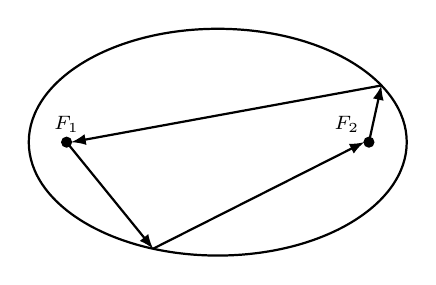
\begin{tikzpicture}[scale=1.2]%[width=1.16\marginparwidth]
\draw [thick] (0,0) circle[x radius=2cm,y radius = 1.2cm];
\filldraw (1.6,0)  circle (1.5pt) node [above left] {\scriptsize $F_2$}
			(-1.6,0)  circle (1.5pt) node [above] {\scriptsize $F_1$};
\draw[->,>=latex,draw={\colorone},thick] (1.6,0) -- ({2*cos(30)},{1.2*sin(30)});
\draw[->,>=latex,draw={\colorone},thick]({2*cos(30)},{1.2*sin(30)}) -- (-1.55,0);
\draw[->,>=latex,draw={\colortwo},thick] (-1.6,0) -- ({2*cos(250)},{1.2*sin(250)});
\draw[->,>=latex,draw={\colortwo},thick]  ({2*cos(250)},{1.2*sin(250)}) -- (1.55,0);
\end{tikzpicture}}

\theorem{thm:ellipse_reflect}{Reflective Property of an Ellipse}
{Let $P$ be a point on a ellipse with foci $F_1$ and $F_2$. The tangent line to the ellipse at $P$ makes equal angles with the following two lines:\index{ellipse!reflective property}
\begin{enumerate}
	\item The line through $F_1$ and $P$, and
	\item The line through $F_2$ and $P$. 
\end{enumerate}}

% todo prove the reflective property of ellipses

This reflective property is useful in optics and is the basis of the phenomena experienced in whispering halls.
}

% todo prove that a parabola is the limiting case of an ellipse

\subsection{Hyperbolas}

The definition of a hyperbola is very similar to the definition of an ellipse; we essentially just change the word ``sum'' to ``difference.''

\definition{def:hyperbola}{Hyperbola}
{A \textbf{hyperbola} is the locus of all points where the absolute value of the difference of distances from two fixed points, each a focus of the hyperbola, is constant.
\index{conic sections!hyperbola}\index{hyperbola!definition}\index{focus}}

We do not have a convenient way of visualizing the construction of a hyperbola as we did for the ellipse. The geometric definition does allow us to find an algebraic expression that describes it. It will be useful to define some terms first.

\mtable{Labeling the significant features of a hyperbola.}{fig:hyperbola_def}{\begin{tikzpicture}
\begin{axis}[width=1.16\marginparwidth,tick label style={font=\scriptsize},
axis y line=none,axis x line=none,name=myplot,
ymin=-3.2,ymax=3.2,xmin=-3.2,xmax=3.2]
\addplot [thick, draw={\colorone},smooth,domain=-70:70,samples=60] ({sec(x)},{tan(x)});
\addplot [thick, draw={\colorone},smooth,domain=-70:70,samples=60] ({-sec(x)},{tan(x)});
\filldraw (axis cs:0,0)  circle (1.5pt);
\draw [thick,dashed] 	(axis cs:-3.2,0)
 --  node [above,pos=.88] {\scriptsize Transverse}
 node [below,pos=.88] {\scriptsize axis}(axis cs:3.2,0)
 (axis cs:0,-3.2)
 -- node [below,rotate=90,pos=.8] {\scriptsize  axis }
 node [above,rotate=90,pos=.8] {\scriptsize Conjugate}(axis cs:0,3.2);
\filldraw [draw={\colorone}] (axis cs:1,0)circle(1.5pt) (axis cs:-1,0)circle(1.5pt);
\filldraw [draw={\colortwo}] (axis cs:1.4,0)circle(1.5pt) node (f1) {}
						(axis cs:-1.4,0)  circle (1.5pt) node (f2) {};
\draw [->,>=latex] (axis cs: 1.25,-2.8) -- (axis cs: -1.35,-.1);
\draw [->,>=latex] (axis cs: 1.25,-2.8) node [fill=white] {\scriptsize Foci }
 -- (axis cs: 1.4,-.1);	
\draw [->,>=latex] (axis cs: -1.25,-2.8) -- (axis cs: -1,-.1);
\draw [->,>=latex] (axis cs: -1.25,-2.8) node [fill=white] {\scriptsize Vertices}
 -- (axis cs: .95,-.1);	
\draw (axis cs:-.5,.4) node {\scriptsize $\overbrace{\rule{18pt}{0pt}}^a$};
\draw (axis cs:.7,.4) node {\scriptsize $\overbrace{\rule{25pt}{0pt}}^c$};
\end{axis}
\end{tikzpicture}}

The two foci lie on the \textbf{transverse axis} of the hyperbola; the midpoint of the line segment joining the foci is the \textbf{center} of the hyperbola. The transverse axis intersects the hyperbola at two points, each a \textbf{vertex} of the hyperbola. The line through the center and perpendicular to the transverse axis is the \textbf{conjugate axis.} This is illustrated in \autoref{fig:hyperbola_def}. It is easy to show that the constant difference of distances used in the definition of the hyperbola is the distance between the vertices, i.e., $2a$.

\keyidea{idea:hyperbola}{Standard Equation of a Hyperbola}
{The equation of a hyperbola centered at $(h,k)$ in standard form is:
\index{hyperbola!standard equation}
\begin{enumerate}
	\item \parbox{120pt}{\textbf{Horizontal Transverse Axis:}} $\ds \frac{(x-h)^2}{a^2} - \frac{(y-k)^2}{b^2} = 1.$
	\item	\parbox{120pt}{\textbf{Vertical Transverse Axis:}} $\ds \frac{(y-k)^2}{a^2}-\frac{(x-h)^2}{b^2} = 1.$
\end{enumerate}
The vertices are located $a$ units from the center and the foci are located $c$ units from the center, where $c^2 = a^2+b^2$.}

\subsection{Graphing Hyperbolas}

\mtable[-1in]{Graphing the hyperbola $\frac{x^2}9-\frac{y^2}1 = 1$ along with its asymptotes, $y=\pm x/3$.}{fig:hyperbola_asy1}{\begin{tikzpicture}
\begin{axis}[width=1.16\marginparwidth,tick label style={font=\scriptsize},
axis y line=middle,axis x line=middle,name=myplot,
ymin=-3.2,ymax=3.2,xmin=-8.2,xmax=8.2]
\addplot [thick, draw={\colorone},smooth,domain=-70:70,samples=60] ({3*sec(x)},{tan(x)});
\addplot [thick, draw={\colorone},smooth,domain=-70:70,samples=60] ({-3*sec(x)},{tan(x)});
\addplot [thick,dashed,draw={\colortwo},domain=-8:8] {x/3};
\addplot [thick,dashed,draw={\colortwo},domain=-8:8] {-x/3};
\end{axis}
\node [right] at (myplot.right of origin) {\scriptsize $x$};
\node [above] at (myplot.above origin) {\scriptsize $y$};
\end{tikzpicture}}

Consider the hyperbola $\frac{x^2}9-\frac{y^2}1 = 1$. Solving for $y$, we find $y=\pm\sqrt{x^2/9-1}$. As $x$ grows large, the ``$-1$'' part of the equation for $y$ becomes less significant and $y\approx \pm\sqrt{x^2/9} = \pm x/3$. That is, as $x$ gets large, the graph of the hyperbola looks very much like the lines $y=\pm x/3$. These lines are asymptotes of the hyperbola, as shown in \autoref{fig:hyperbola_asy1}.

\mtable{Using the asymptotes of a hyperbola as a graphing aid.}{fig:hyperbola_asy2}{\begin{tikzpicture}
\begin{axis}[width=1.16\marginparwidth,tick label style={font=\scriptsize},
axis y line=middle,axis x line=middle,name=myplot,xtick=\empty,extra x ticks={2,8,5},
extra x tick labels={$h-a$, $h+a$,$h$},ytick=\empty,extra y ticks={2,4,6},
extra y tick labels={$k-b$, $k$, $k+b$},ymin=-2.2,ymax=10.2,xmin=-3.2,xmax=13.2]
\addplot [thick, draw={\colorone},smooth,domain=-70:70,samples=60]
 ({3*sec(x)+5},{2*tan(x)+4});
\addplot [thick, draw={\colorone},smooth,domain=-70:70,samples=60]
 ({-3*sec(x)+5},{2*tan(x)+4});
\draw [thick,dashed] (axis cs: 2,6) -- (axis cs:8,6) -- (axis cs:8,2)
 -- (axis cs: 2,2) -- cycle;
\addplot [thick,dashed,draw={\colortwo},domain=-3:13] {2*(x-5)/3+4};
\addplot [thick,dashed,draw={\colortwo},domain=-3:13] {-2*(x-5)/3+4};
\filldraw (axis cs:5,4) circle (1.5pt);
\filldraw [draw={\colorone}] (axis cs:2,4) circle (1.5pt);
\filldraw [draw={\colorone}] (axis cs:8,4) circle (1.5pt);
\end{axis}
\node [right] at (myplot.right of origin) {\scriptsize $x$};
\node [above] at (myplot.above origin) {\scriptsize $y$};
\end{tikzpicture}}

This is a valuable tool in sketching. Given the equation of a hyperbola in general form, draw a rectangle centered at $(h,k)$ with sides of length $2a$ parallel to the transverse axis and sides of length $2b$ parallel to the conjugate axis. (See \autoref{fig:hyperbola_asy2} for an example with a horizontal transverse axis.) The diagonals of the rectangle lie on the asymptotes. 

These lines pass through $(h,k)$.  When the transverse axis is horizontal, the slopes are $\pm b/a$; when the transverse axis is vertical, their slopes are $\pm a/b$. This gives equations:
\begin{center}
\begin{tabular}{cc}
\parbox{100pt}{\centering Horizontal \\ Transverse Axis} & \parbox{100pt}{\centering Vertical \\ Transverse Axis} \\ \ \\
$\ds y=\pm\frac ba(x-h)+k$  &$\ds  y=\pm\frac ab(x-h)+k.$
\end{tabular}
\end{center}

\mtable{Graphing the hyperbola in \autoref{ex_conic5}.}{fig:conic5}{\begin{tikzpicture}
\begin{axis}[width=1.16\marginparwidth,tick label style={font=\scriptsize},
axis y line=middle,axis x line=middle,name=myplot,minor x tick num=4,
minor y tick num=4,ymin=-7.2,ymax=11.2,xmin=-5.2,xmax=7.2]
\addplot [thick, draw={\colorone},smooth,domain=-70:70,samples=60]
 ({2*tan(x)+1},{5*sec(x)+2});
\addplot [thick, draw={\colorone},smooth,domain=-70:70,samples=60]
 ({2*tan(x)+1},{-5*sec(x)+2});
\draw [thick,dashed] (axis cs: -1,7) -- (axis cs:3,7) -- (axis cs:3,-3)
 -- (axis cs: -1,-3) -- cycle;
\addplot [thick,dashed,draw={\colortwo},domain=-3:13] {5*(x-1)/2+2};
\addplot [thick,dashed,draw={\colortwo},domain=-3:13] {-5*(x-1)/2+2};
\filldraw (axis cs:1,2) circle (1.5pt);
\filldraw [draw={\colorone}] (axis cs:1,7) circle (1.5pt);
\filldraw [draw={\colorone}] (axis cs:1,-3) circle (1.5pt);
\filldraw [draw={\colortwo}] (axis cs:1,7.4) circle (1.5pt);
\filldraw [draw={\colortwo}] (axis cs:1,-3.4) circle (1.5pt);
\end{axis}
\node [right] at (myplot.right of origin) {\scriptsize $x$};
\node [above] at (myplot.above origin) {\scriptsize $y$};
\end{tikzpicture}}

\example{ex_conic5}{Graphing a hyperbola}{Sketch the hyperbola given by $\ds \frac{(y-2)^2}{25}-\frac{(x-1)^2}{4}=1.$}
{The hyperbola is centered at $(1,2)$; $a=5$ and $b=2$.
In \autoref{fig:conic5} we draw the prescribed rectangle centered at $(1,2)$ along with the asymptotes defined by its diagonals. The hyperbola has a vertical transverse axis, so the vertices are located at $(1,7)$ and $(1,-3)$. This is enough to make a good sketch.

We also find the location of the foci: as $c^2= a^2+b^2$, we have $c=\sqrt{29}\approx 5.4$. Thus the foci are located at $(1,2\pm 5.4)$ as shown in the figure.}

\mtable{Graphing the hyperbola in \autoref{ex_conic6}.}{fig:conic6}{\begin{tikzpicture}
\begin{axis}[width=1.16\marginparwidth,tick label style={font=\scriptsize},
axis y line=middle,axis x line=middle,name=myplot,minor x tick num=1,
minor y tick num=4,ymin=-10.9,ymax=11.9,xmin=-4.2,xmax=4.2]
\addplot [thick, draw={\colorone},smooth,domain=-75:75,samples=60]
 ({sec(x)},{3*tan(x)+1});
\addplot [thick, draw={\colorone},smooth,domain=-75:75,samples=60]
 ({-sec(x)},{3*tan(x)+1});
\draw [thick,dashed] (axis cs: -1,4) -- (axis cs:1,4) -- (axis cs:1,-2)
 -- (axis cs: -1,-2) -- cycle;
\addplot [thick,dashed,draw={\colortwo},domain=-4:4] {3*(x-0)/1+1};
\addplot [thick,dashed,draw={\colortwo},domain=-4:4] {-3*(x-0)/1+1};
\filldraw (axis cs:0,1) circle (1.5pt);
\filldraw [draw={\colorone}] (axis cs:-1,1) circle (1.5pt);
\filldraw [draw={\colorone}] (axis cs:1,1) circle (1.5pt);
\filldraw [draw={\colortwo}] (axis cs:3.2,1) circle (1.5pt);
\filldraw [draw={\colortwo}] (axis cs:-3.2,1) circle (1.5pt);
\end{axis}
\node [right] at (myplot.right of origin) {\scriptsize $x$};
\node [above] at (myplot.above origin) {\scriptsize $y$};
\end{tikzpicture}}

\example{ex_conic6}{Graphing a hyperbola}{Sketch the hyperbola given by $9x^2-y^2+2y=10.$}
{We must complete the square to put the equation in general form. (We recognize this as a hyperbola since it is a general quadratic equation and the $x^2$ and $y^2$ terms have opposite signs.)
\begin{align*}
	9x^2-y^2+2y &=10\\
	9x^2- (y^2-2y) &= 10\\
	9x^2 - (y^2-2y+1-1) &= 10\\
	9x^2 -\big((y-1)^2-1\big) &= 10\\
	9x^2 - (y-1)^2 &= 9\\
	x^2 - \frac{(y-1)^2}{9} &=1
\end{align*}

We see the hyperbola is centered at $(0,1)$, with a horizontal transverse axis, where $a=1$ and $b=3$. The appropriate rectangle is sketched in \autoref{fig:conic6} along with the asymptotes of the hyperbola. The vertices are located at $(\pm 1,1)$. We have $c=\sqrt{10}\approx 3.2$, so the foci are located at $(\pm 3.2,1)$ as shown in \autoref{fig:conic6}.}

\ifthenelse{\boolean{abridgeConics}}{}{%
\subsection{Eccentricity}

\definition{def:hyperbola_eccentricity}{Eccentricity of a Hyperbola}
{The eccentricity of a hyperbola is $\ds e=\frac ca$.\index{hyperbola!eccentricity}\index{eccentricity}}

Note that this is the definition of eccentricity as used for the ellipse.  When $c$ is close in value to $a$ (i.e., $e\approx 1$), the hyperbola is very narrow (looking almost like crossed lines). \autoref{fig:hyperbola_ecc} shows hyperbolas centered at the origin with $a=1$. The graph in (a) has $c=1.05$, giving an eccentricity of $e=1.05$, which is close to 1. As $c$ grows larger, the hyperbola widens and begins to look like parallel lines, as shown in part (d) of the figure.

\begin{lxfigure}
 \begin{tabular}{cc}
\begin{tikzpicture}
\begin{axis}[width=1.16\marginparwidth,tick label style={font=\scriptsize},
axis y line=middle,axis x line=middle,name=myplot,xtick={-10,-5,5,10},
minor x tick num=4,ytick={-10,-5,5,10},minor y tick num=4,
ymin=-11.9,ymax=11.9,xmin=-11.9,xmax=11.9,axis equal]
\addplot [thick, draw={\colorone},smooth,domain=-85:85,samples=60]
 ({sec(x)},{.32*tan(x)});
\addplot [thick, draw={\colorone},smooth,domain=-85:85,samples=60]
 ({-sec(x)},{.32*tan(x)});
\filldraw (axis cs:0,0) circle (1.5pt);
\filldraw [draw={\colorone}] (axis cs:-1,0) circle (1.5pt);
\filldraw [draw={\colorone}] (axis cs:1,0) circle (1.5pt);
\filldraw [draw={\colortwo}] (axis cs:1.05,0) circle (1.5pt);
\filldraw [draw={\colortwo}] (axis cs:-1.05,0) circle (1.5pt);
\draw (axis cs: 9,-6) node {\scriptsize $e = 1.05$};					
\end{axis}
\node [right] at (myplot.right of origin) {\scriptsize $x$};
\node [above] at (myplot.above origin) {\scriptsize $y$};
\end{tikzpicture}
  &
\begin{tikzpicture}
\begin{axis}[width=1.16\marginparwidth,tick label style={font=\scriptsize},
axis y line=middle,axis x line=middle,name=myplot,xtick={-10,-5,5,10},
minor x tick num=4,ytick={-10,-5,5,10},minor y tick num=4,
ymin=-11.9,ymax=11.9,xmin=-11.9,xmax=11.9,axis equal]
\addplot [thick, draw={\colorone},smooth,domain=-85:85,samples=60]
 ({sec(x)},{1.12*tan(x)});
\addplot [thick, draw={\colorone},smooth,domain=-85:85,samples=60]
 ({-sec(x)},{1.12*tan(x)});
\filldraw (axis cs:0,0) circle (1.5pt);
\filldraw [draw={\colorone}] (axis cs:-1,0) circle (1.5pt);
\filldraw [draw={\colorone}] (axis cs:1,0) circle (1.5pt);
\filldraw [draw={\colortwo}] (axis cs:1.5,0) circle (1.5pt);
\filldraw [draw={\colortwo}] (axis cs:-1.5,0) circle (1.5pt);
\draw (axis cs: 9,-6) node {\scriptsize $e = 1.5$};					
\end{axis}
\node [right] at (myplot.right of origin) {\scriptsize $x$};
\node [above] at (myplot.above origin) {\scriptsize $y$};
\end{tikzpicture}
  \\(a)&(b) \\
\begin{tikzpicture}
\begin{axis}[width=1.16\marginparwidth,tick label style={font=\scriptsize},
axis y line=middle,axis x line=middle,name=myplot,xtick={-10,-5,5,10},
minor x tick num=4,ytick={-10,-5,5,10},minor y tick num=4,
ymin=-11.9,ymax=11.9,xmin=-11.9,xmax=11.9,axis equal]
\addplot [thick, draw={\colorone},smooth,domain=-85:85,samples=60]
 ({sec(x)},{2.83*tan(x)});
\addplot [thick, draw={\colorone},smooth,domain=-85:85,samples=60]
 ({-sec(x)},{2.83*tan(x)});
\filldraw (axis cs:0,0) circle (1.5pt);
\filldraw [draw={\colorone}] (axis cs:-1,0) circle (1.5pt);
\filldraw [draw={\colorone}] (axis cs:1,0) circle (1.5pt);
\filldraw [draw={\colortwo}] (axis cs:3,0) circle (1.5pt);
\filldraw [draw={\colortwo}] (axis cs:-3,0) circle (1.5pt);
\draw (axis cs: 9,-6) node {\scriptsize $e = 3$};					
\end{axis}
\node [right] at (myplot.right of origin) {\scriptsize $x$};
\node [above] at (myplot.above origin) {\scriptsize $y$};
\end{tikzpicture}
  &
\begin{tikzpicture}
\begin{axis}[width=1.16\marginparwidth,tick label style={font=\scriptsize},
axis y line=middle,axis x line=middle,name=myplot,xtick={-10,-5,5,10},
minor x tick num=4,ytick={-10,-5,5,10},minor y tick num=4,
ymin=-11.9,ymax=11.9,xmin=-11.9,xmax=11.9,axis equal]
\addplot [thick, draw={\colorone},smooth,domain=-85:85,samples=60] ({sec(x)},{9.95*tan(x)});
\addplot [thick, draw={\colorone},smooth,domain=-85:85,samples=60] ({-sec(x)},{9.95*tan(x)});
\filldraw (axis cs:0,0) circle (1.5pt);
\filldraw [draw={\colorone}] (axis cs:-1,0) circle (1.5pt);
\filldraw [draw={\colorone}] (axis cs:1,0) circle (1.5pt);
\filldraw [draw={\colortwo}] (axis cs:10,0) circle (1.5pt);
\filldraw [draw={\colortwo}] (axis cs:-10,0) circle (1.5pt);
\draw (axis cs: 9,-6) node {\scriptsize $e = 10$};					
\end{axis}
\node [right] at (myplot.right of origin) {\scriptsize $x$};
\node [above] at (myplot.above origin) {\scriptsize $y$};
\end{tikzpicture}
  \\(c)&(d)
 \end{tabular}
 \caption{Understanding the eccentricity of a hyperbola.}
 \label{fig:hyperbola_ecc}
\end{lxfigure}

\subsection{Reflective Property}

Hyperbolas share a similar reflective property with ellipses. However, in the case of a hyperbola, a ray emanating from a focus that intersects the hyperbola reflects along a line containing the other focus, but moving \textit{away} from that focus. This is illustrated in \autoref{fig:hyperbola_reflect} (on the next page). Hyperbolic mirrors are commonly used in telescopes because of this reflective property. It is stated formally in the following theorem.

\theorem{thm:reflective_hyperbola}{Reflective Property of Hyperbolas}
{Let $P$ be a point on a hyperbola with foci $F_1$ and $F_2$. The tangent line to the hyperbola at $P$ makes equal angles with the following two lines:\index{hyperbola!reflective property}
\begin{enumerate}
	\item	The line through $F_1$ and $P$, and
	\item	The line through $F_2$ and $P$.
\end{enumerate}}

% todo prove the reflective property of hyperbolas

% todo prove that a parabola is the limiting case of a hyperbola

\subsection{Location Determination}

Determining the location of a known event has many practical uses (locating the epicenter of an earthquake, an airplane crash site, the position of the person speaking in a large room, etc.).

To determine the location of an earthquake's epicenter, seismologists use \textit{trilateration} (not to be confused with \textit{triangulation}). A seismograph allows one to determine how far away the epicenter was; using three separate readings, the location of the epicenter can be approximated.

A key to this method is knowing distances. What if this information is not available? Consider three microphones at positions $A$, $B$ and $C$ which all record a noise (a person's voice, an explosion, etc.) created at unknown location $D$. The microphone does not ``know'' when the sound was \textit{created}, only when the sound was \textit{detected}. How can the location be determined in such a situation?

\mtable{Illustrating the reflective property of a hyperbola.}{fig:hyperbola_reflect}{\begin{tikzpicture}
\begin{axis}[width=1.16\marginparwidth,tick label style={font=\scriptsize},
axis y line=none,axis x line=none,name=myplot,
ymin=-11.9,ymax=11.9,xmin=-5,xmax=5]
\addplot [thick, smooth,domain=-85:85,samples=60] ({sec(x)},{2.83*tan(x)});
\addplot [thick,smooth,domain=-85:85,samples=60] ({-sec(x)},{2.83*tan(x)});
\filldraw (axis cs:0,0) circle (1.5pt);
\filldraw [draw={\colorone}] (axis cs:-1,0) circle (1.5pt);
\filldraw [draw={\colorone}] (axis cs:1,0) circle (1.5pt);
\draw [draw={\colortwo},thick,->,>=latex] (axis cs:-3,0) -- (axis cs: 1.4,2.83);
\draw [draw={\colortwo},thick,->,>=latex] (axis cs:1.4,2.83)--(axis cs: -1.8,8.49);
\draw [dashed,draw={\colortwo},thick] (axis cs:1.4,2.83)--(axis cs: 3,0);
\filldraw [] (axis cs:1.4,2.83) circle (1.5pt);
\filldraw [] (axis cs:3,0) circle (1.5pt) node [below] {\scriptsize $F_2$};
\filldraw [] (axis cs:-3,0) circle (1.5pt) node [below] {\scriptsize $F_1$};
\end{axis}
\end{tikzpicture}}

If each location has a clock set to the same time, hyperbolas can be used to determine the location. Suppose the microphone at position $A$ records the sound at exactly 12:00, location $B$ records the time exactly 1 second later, and location $C$ records the noise exactly 2 seconds after that. We are interested in the \textit{difference} of times. Since the speed of sound is approximately 340 m/s, we can conclude quickly that the sound was created 340 meters closer to position $A$ than position $B$. If $A$ and $B$ are a known distance apart (as shown in \autoref{fig:hyperbola_locate} (a)), then we can determine a hyperbola on which $D$ must lie. 

The ``difference of distances'' is 340; this is also the distance between vertices of the hyperbola. So we know $2a=340$. Positions $A$ and $B$ lie on the foci, so $2c=1000$. From this we can find $b\approx 470$ and can sketch the hyperbola, given in part (b) of the figure. We only care about the side closest to $A$. (Why?)

We can also find the hyperbola defined by positions $B$ and $C$. In this case, $2a = 680$ as the sound traveled an extra 2 seconds to get to $C$. We still have $2c=1000$, centering this hyperbola at $(-500,500)$. We find $b\approx 367$. This hyperbola is sketched in part (c) of the figure. The intersection point of the two graphs is the location of the sound, at approximately $(188,-222.5)$.

\begin{lxfigure}
\flushinner{%
\begin{tabular}{c @{\hspace{1em}} c @{\hspace{1em}} c}
\begin{tikzpicture}
\begin{axis}[width=1.16\marginparwidth,tick label style={font=\scriptsize},
axis y line=middle,axis x line=middle,name=myplot,
ymin=-1100,ymax=1100,xmin=-1100,xmax=1100]
\filldraw (axis cs:500,0) circle (1.5pt) node [above] {\scriptsize $A$};
\filldraw (axis cs:-500,0) circle (1.5pt) node [above] {\scriptsize $B$};
\filldraw (axis cs:-500,1000) circle (1.5pt) node [left] {\scriptsize $C$};
\end{axis}
\end{tikzpicture}
 &
\begin{tikzpicture}
\begin{axis}[width=1.16\marginparwidth,tick label style={font=\scriptsize},
axis y line=middle,axis x line=middle,name=myplot,
ymin=-1100,ymax=1100,xmin=-1100,xmax=1100]
\addplot [thick, smooth,domain=-85:85,samples=60] ({170*sec(x)},{470*tan(x)});
\addplot [dashed,thick,smooth,domain=-85:85,samples=60] ({-170*sec(x)},{470*tan(x)});
\filldraw (axis cs:500,0) circle (1.5pt) node [above] {\scriptsize $A$};
\filldraw (axis cs:-500,0) circle (1.5pt) node [above] {\scriptsize $B$};
\filldraw (axis cs:-500,1000) circle (1.5pt) node [left] {\scriptsize $C$};
\end{axis}
\end{tikzpicture}
 &
\begin{tikzpicture}
\begin{axis}[width=1.16\marginparwidth,tick label style={font=\scriptsize},
axis y line=middle,axis x line=middle,name=myplot,
ymin=-1100,ymax=1100,xmin=-1100,xmax=1100]
\addplot [thick, smooth,domain=-85:85,samples=60] ({170*sec(x)},{470*tan(x)});
\addplot [dashed,thick, smooth,domain=-85:85,samples=60]
 ({367*tan(x)-500},{340*sec(x)+500});
\addplot [thick, smooth,domain=-85:85,samples=60]
 ({367*tan(x)-500},{-340*sec(x)+500});
\filldraw (axis cs:500,0) circle (1.5pt) node [above] {\scriptsize $A$};
\filldraw (axis cs:-500,0) circle (1.5pt) node [above] {\scriptsize $B$};
\filldraw (axis cs:-500,1000) circle (1.5pt) node [left] {\scriptsize $C$};
\filldraw (axis cs:188,-222) circle (1.5pt) node [below left] {\scriptsize $D$};
\end{axis}
\end{tikzpicture}
\\(a) & (b) & (c)
\end{tabular}}
\caption{Using hyperbolas in location detection.}%
\label{fig:hyperbola_locate}
\end{lxfigure}
}

This chapter explores curves in the plane, in particular curves that cannot be described by functions of the form $y=f(x)$. In this section, we learned of ellipses and hyperbolas that are defined implicitly, not explicitly. In the following sections, we will learn completely new ways of describing curves in the plane, using \emph{parametric equations} and \emph{polar coordinates}, then study these curves using calculus techniques.

\printexercises{exercises/09_01_exercises}
